\definecolor{specorange}{HTML}{FE8010}
\definecolor{taublue}{HTML}{468FD8}
\definecolor{trapgreen}{HTML}{70AD47}
\definecolor{directgray}{HTML}{404040}

\begin{figure}[t]

\begin{minipage}[c]{0.45\textwidth}
\centering
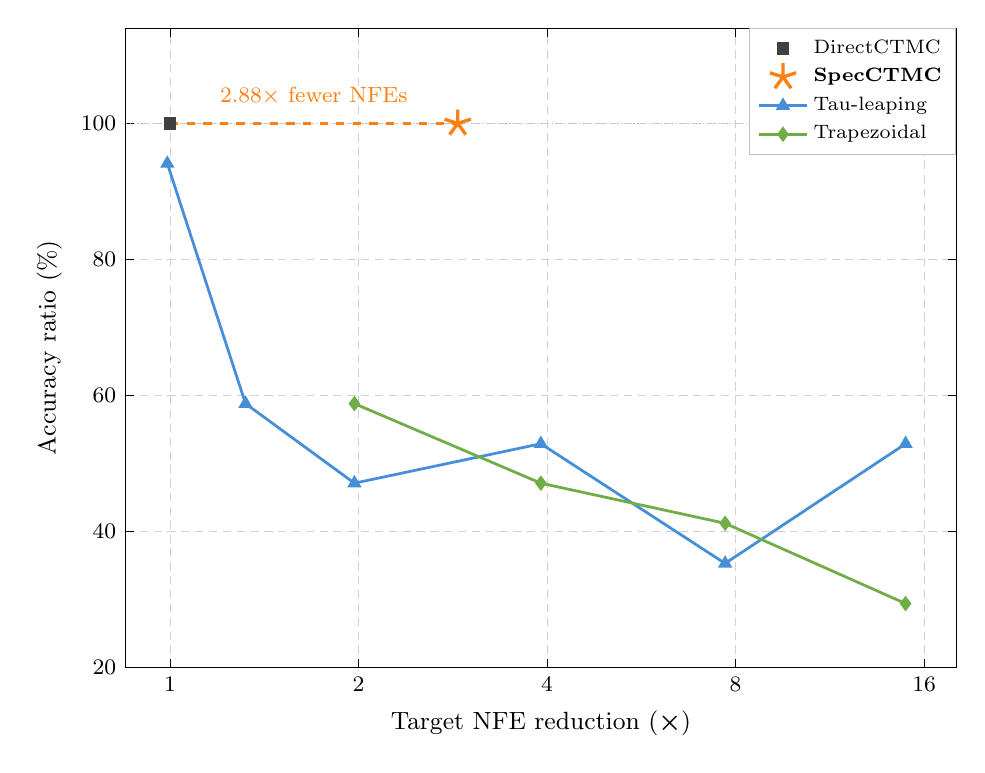
\begin{tikzpicture}
\begin{axis}[
    width=\linewidth,
    height=0.8\linewidth,
    % title={LLaDA-8B-Instruct / GSM8K},
    % title style={font=\small\bfseries},
    xlabel={Target NFE reduction ($\times$)},
    ylabel={Accuracy ratio (\%)},
    label style={font=\small\boldmath},
    tick label style={font=\footnotesize},
    xmode=log,
    log basis x=2,
    xmin=0.85, xmax=18,
    xtick={1,2,4,8,16},
    xticklabels={1,2,4,8,16},
    ymin=20, ymax=114,
    ytick={20,40,60,80,100},
    minor x tick num=0,
    % axis lines=left,
    axis line style={black},
    tick style={black},
    tick align=inside,
    major tick length=3pt,
    ymajorgrids=true,
    xmajorgrids=true,
    grid style={densely dashed,black!18},
    clip=false,
    legend style={
        at={(1.00,1.00)},
        anchor=north east,
        legend columns=1,
        draw=black!25,
        fill=white!50,
        font=\scriptsize,
        /tikz/every even column/.append style={column sep=3pt},
    },
    legend cell align=left,
]

% Reference accuracy.
\addplot[
    gray!55,
    densely dotted,
    thin,
    forget plot,
] coordinates {(0.85,100) (18,100)};

% Direct-CTMC.
\addplot[
    only marks,
    color=directgray,
    mark=square*,
    mark size=2pt,
] coordinates {(1,100)};
\addlegendentry{DirectCTMC}

% Spec-CTMC: open star denotes retention in expectation.
\addplot[
    only marks,
    color=specorange,
    mark=star,
    mark size=5pt,
    mark options={solid,line width=1.2pt},
] coordinates {(2.88,100)};
\addlegendentry{\bf SpecCTMC}

% Horizontal comparison arrow; midpoint is centered in log-axis display space.
\draw[color=specorange,dashed,line width=0.9pt,]
      % shorten <=2pt,shorten >=2pt]
    (axis cs:1,100) --
    node[midway,above=3pt,font=\footnotesize,text=specorange]
        {$2.88\times$ fewer NFEs}
    (axis cs:2.88,100);

% Tau-leaping.
% Solver step counts retained in source data; labels hidden.
\addplot[
    color=taublue,
    solid,
    line width=1pt,
    mark=triangle*,
    mark size=2pt,
    point meta=explicit symbolic,
] table[
    x=reduction,
    y=retained,
    meta=steps,
    row sep=\\,
] {
    reduction retained steps \\
    0.99      94.1     256   \\
    1.32      58.8     192   \\
    1.97      47.1     128   \\
    3.91      52.9     64    \\
    7.70      35.3     32    \\
    14.95     52.9     16    \\
};
\addlegendentry{Tau-leaping}

% Trapezoidal sampling: reference blue.
\addplot[
    color=trapgreen,
    solid,
    line width=1pt,
    mark=diamond*,
    mark size=2pt,
    point meta=explicit symbolic,
] table[
    x=reduction,
    y=retained,
    meta=steps,
    row sep=\\,
] {
    reduction retained steps \\
    1.97      58.8     64    \\
    3.91      47.1     32    \\
    7.70      41.2     16    \\
    14.95     29.4     8     \\
};
\addlegendentry{Trapezoidal}

\end{axis}
\end{tikzpicture}
\end{minipage}

\caption{
{\bf Exact law preserving of \method on NFE acceleration.} On GSM8K with LLaDA-8B-Instruct (256 generated tokens), SpecCTMC reduces target NFEs by $2.88\times$ relative to DirectCTMC while preserving expected accuracy. Finite-step samplers trade accuracy for fewer evaluations.
}

\label{fig:intro-tradeoff}
\end{figure}